%"Individual Monitors" is part two of the section "Smart Breakers", preceeded by "Breakers"

\subsection{Individual Monitor}
\subsubsection{Problem Definition}
The individual circuit monitors provide the means for the homeowner to know where power is used within the building and makes up the second half of the smart breakers, along with the switching circuitry. They measure voltage and current in the connected home circuit, use it for controlling the breakers and feed the information to the user through the base station. Homeowners can then use the information to adjust their power consumption habits, while the control logic uses the information to detect over-current and over-voltage situations and change the switch's status accordingly. 

\subsubsection{System Diagram}
\begin{figure}[htbp]
\begin{center}
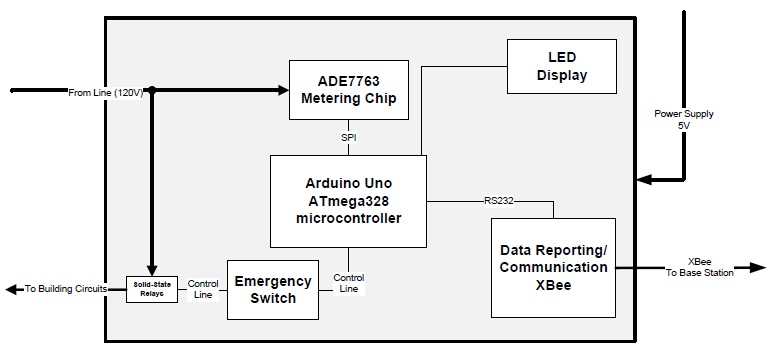
\includegraphics[width=6in]{includes/NJSmartBreakerMonitor}
\caption{Detailed block diagram of monitoring part of the Smart Breakers}
\label{fig:monitor_system_diagram}
\end{center}
\end{figure}

The above diagram shows the components of the individual monitors and their relationships to each other and the breaker section of the smart breakers. 

\subsubsection{System Components}
Metering Chip

The purpose of the metering chip and its inputs is to measure instantaneous voltage and current as it enters the home and pass the data to the controller. 

At the beginning of the year, the team found ADE7763 metering chips from Analog Devices and obtained free samples. As an IC designed for energy metering \cite{ADE7763}, the chip has all of the functionality needed for the project. At a minimum, the chip needs to read voltage and current with additional measurements being nice but not necessary. The team also found several other chips that perform similarly, but due to cost to the design team, the ADE7763 metering chips were used. The team recognizes this is not good customer driven design, but for proving that metering is feasible at the individual circuit level, the decision was acceptable.

Input methods for the ADE7763 were selected based on the AN 564 app note \cite{AN564}, using a current transformer and voltage divider to measure the power line. Both work well for the project because they are simple and accurate. The team had originally hoped to keep the cost to the consumer below \$20 so that replacing an average of 20 standard air-gap breakers would cost less than \$400, which is comparable to similar products (see Business Competition section for more). The high turns ratio current transformer's cost of \$14.23 pushes the smart breaker cost to \$10 more than originallly hoped, but was easily available. An alternative considered after the decision to purchase the high turns ratio current transformer was a lower turns ratio current transformer at a lower cost, combined with a voltage divider. However, implementing this would have used up more of the budget, which the team wanted to save for other aspects of the project. The voltage divider is both easily available and low cost, although it does not provide good protection against lightning strikes, which could present a problem since replacing only one individual component of the smart breaker is not feasible. Selected components and values keep the input levels lower than the maximum value of 500 \milli\volt \cite{ADE7763} for the ADE7763 channels using the equations below.

\begin{equation} % Eq. 1
V_{secondary}=\frac{(I_{primary}*R_{burden})}{2511}
\label{eq:v_secondary}
\end{equation}

This gives the voltage across the secondary of the current transformer and comes from the datasheet for the current transformer \cite{CT_nate}. From this equation, $R_{burden}$ is selected as $60 \ohm$, allowing the current transformer to be used for up to $20\ampere$.

\begin{equation} % Eq. 2
V_{measure}=V_{line}*\frac{R_{measure}}{R_{total}}
\label{eq:volt_divider}
\end{equation}

\begin{equation} % Eq. 3
P=\frac{V^2}{R}
\label{eq:power1}
\end{equation}

Equation \ref{eq:volt_divider} is the standard voltage divider equation used to determine values so the maximum input voltage is not exceeded. Equation \ref{eq:power1} is the power equation used to determine resistor values so they don't draw too much power. To keep $V_{measure}$ under $500\milli \V$, $R_{measure}$ is $1\kilo\ohm$ with an $R_{total}$ of $511\kilo\ohm$. 

\begin{equation} % Eq. 4
f_{3dB}=\frac{1}{(2*pi*R*C)}
\label{eq:low_pass}
\end{equation}

Equation \ref{eq:low_pass} is used to determine the 3dB point of the attenuation network in Figure \ref{fig:attenuation_network} (an-564). A $22\nano\farad$ capacitor with the $R_{measure}$ from above gives a cutoff of $7200\hertz$ as suggested by the app note \cite{AN564}. 

\begin{figure}[htbp]
\begin{center}
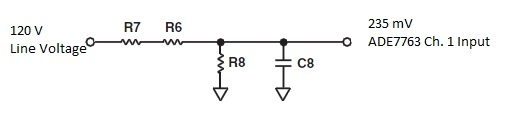
\includegraphics[width=4in]{includes/NJAttenuationNetwork2} 
\caption{Attenuation network for ADE7763 \cite{AN564}}
\label{fig:attenuation_network} 
\end{center}
\end{figure}

Microcontroller

The microcontroller's job is to transfer the data stored in the metering chip's registers to the base station and does so through the SPI connection built into the chip. It also provides the logic needed to detect and turn off the breaker in an over-voltage or over-current situation. Other functions include managing start up and shut down, primarily initializing registers and saving data. 

\begin{equation} % Eq. 5
V_{voltageMax}=V_{line}*\frac{R_{measure}}{R_{total}}*N_{safetyFactor}
\label{eq:volt_divide_safety}
\end{equation}

\begin{equation} % Eq. 6
V_{currentMax}=\frac{(I_{limit}*R_{burden})}{2511}*N_{safetyFactor}
\label{eq:current_safety}
\end{equation}

The manufacturers of the smart breakers would use equations \ref{eq:volt_divide_safety} and \ref{eq:current_safety} to determine the exact resistor values based on the desired part ratings. Both $V_{voltageMax}$ and $V_{currentMax}$ equal 500 mV, as specified by the datasheet \cite{ADE7763} and $N_{safetyFactor}$ is a value greater than 1 which the team decided to be 2 and 1.5 for voltage and current respectively. This allows spikes up to 30 A for current and 255 V for voltage without damage to the chip. To determine the threshold values, the resistor values from equations \ref{eq:volt_divide_safety} and \ref{eq:current_safety} are put into equations \ref{eq:v_secondary} and \ref{eq:volt_divider}, giving the analog values for the microcontroller to use.

First semester, the team decided to use an FPGA for this purpose as they are very flexible and can easily manage data from the metering chip. The decision did not meet the criteria of low cost, but was justified by the higly flexible nature and availability. However, the design process for the rest of the breakers took longer than anticipated and the team decided to use the Altera Nios II processor available from Calvin. The team wanted to use the DE2 board to start testing while they continued to decide on a part for a final production design. Calvin also had some pic microcontrollers, but the team is not familiar with them and would have had to learn new protocols and language, making the design more complex than the Nios II which had been used in other classes before. After working with the Nios II function alt\_avalon\_spi\_command(,,,,,,), the team discovered there is very little documentation for the function, making it very difficult to work with and no alternative was found for using SPI. The team decided to look at possible alternative microcontrollers and found an Arduino Uno that uses an ATmega328 microcontroller and has more and clearer documentation. The team used the SPI.transfer() function to pass information, with full code in Appendix \ref{sec:breaker_appendix1} This allowed the team to begin testing, although a cost comparison on the microcontroller for final production has not been completed yet.

Communication

The purpose of the communication component is to transfer data from the smart breakers to the base station and is controlled by the microcontroller. 

First semester the team decided to use Ethernet to achieve this, based on compatibility with the base station, low cost and ability to connect several breakers. However, longer than expected design time for other aspects of the project made it necessary to use a simpler method. The team chose XBee radios instead, transmitting wirelessly with an RS232 connection to the individual components. XBee also removes the need to have external wires connecting the breakers and base station, making the product more aesthetically appealing to the customer in addition to providing a safer installation. 

Display

The purpose of the display is to provide the user with basic on/off information relating to the breakers should the system fail and require a manual shutoff. This meant it must be simple and easy to understand, which led to the decision to use well-labeled LEDs. Because LEDs are very easy to include in a schematic, using them instead of a character-based display also reduced design time.  

Controls

Because it can be critical to shut off power, the team decided to include a physical failsafe method in addition to the system's ability to do so automatically. Because of the way the automatic switching is configured, this backup switch would only allow the user to turn power off. The team decided to eliminate the option to override the automatic controls and force an over-voltage or over-current situation to protect the user if they haven't actually cleared the fault.

\subsubsection{Software}

\begin{figure}[htbp]
\begin{center}
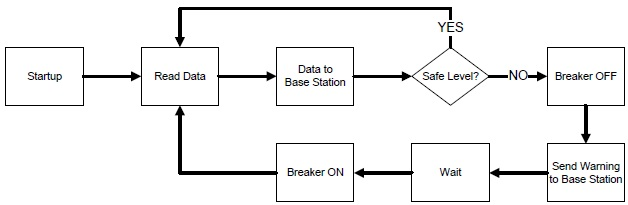
\includegraphics[width=6in]{includes/NJArduinoSoftware2}
\caption{Software flow diagram for Arduino microcontroller}
\label{fig:arduino_software_flow}
\end{center}
\end{figure}

\begin{figure}[htbp]
\begin{center}
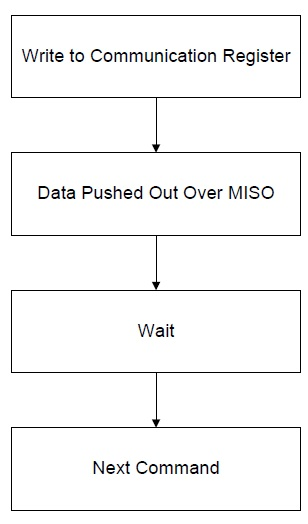
\includegraphics[width=1.5in]{includes/NJADEread2} 
\caption{Read/write process for ADE7763}
\label{fig:ade_read}   
\end{center}
\end{figure}

Figure \ref{fig:arduino_software_flow} shows the microcontroller's operating process for normal operation and what it does in both an over-voltage and over-current situation. Because the purpose of the breaker is to shut off power when unsafe conditions are detected, this is the first thing it does. Since the cause of the unsafe condition is unlikely to remove itself automatically, the smart breaker then alerts the user so they can address the cause. In future work this alert routine may be modified so the user is not overwhelmed with alerts if they do not immediately see the early warnings. The system then waits before taking further action, allowing the user time to clear the cause. Again in future work, this routine may be modified so it waits for a longer period of time if more time has passed since the unsafe condition was initially detected. The last part of the loop for when an unsafe condition is detected is turning the breaker back on. Even if the fault has not been cleared yet, this is a necessary step if the breakers are able to automatically reset since they have no other way of measuring current. This does pose a risk to the user since it allows the over-voltage or over-current condition to continue, but with the line voltage at 60 Hz the system will be able to shut down again within 0.05 seconds, assuming 3 cycles to obtain a reading. The team decided that 3 cycles would provide accurate data without exposing the user to unnecessary danger. 

Voltage and current are both necessary to calculate power, so the team focused on reading those values first. Other features of the ADE7763 may be used if the project were given more time, but as they're not critical, the team didn't deal with them since the ADE7763 makes it easy to ignore information it collects. Some features would include line frequency, apparent and real energy, and possibly sag.

Figure \ref{fig:ade_read} is an expanded view of the read operation in Figure \ref{fig:arduino_software_flow}. According to the datasheet \cite{ADE7763}, a read operation is specified by a zero, followed by the register to be read. However, during testing of the microcontroller, this only returned meaningless data.

\subsubsection{Final Decisions}
To summarize, the individual circuit monitors consist of an Arduino Uno microcontroller and Analog Devices ADE7763 metering chip with input networks using a voltage divider and current transformer. The unit will communicate with the base station computer through the Arduino to computer interface directly, using SPI for communication between the ADE7763 and Arduino Uno. Minimal on/off displays and controls including LEDs and a physical switch will be provided to ensure user safety as well. The system will use a solid state relay to demonstrate that the microcontroller is able to control a switching device, but will use a yet to be determined technology for a marketable product.

\subsubsection{Printed Circuit Board}
The team designed a printed circuit board for the purpose of displaying and testing the prototype design of the smart breakers. It uses parts listed in the Bill of Materials found in the business section and follows the schematic and layout (figures \ref{fig:ade_schematic} and \ref{fig:ade_layout}). After having the board printed and populating it, some initial tests were run, during which a connection exploded, making the board unusable. A second version with a few minor modifications was laid out and put on vector board to replace the first version since the team did not have time to reprint a full board for version two. 

%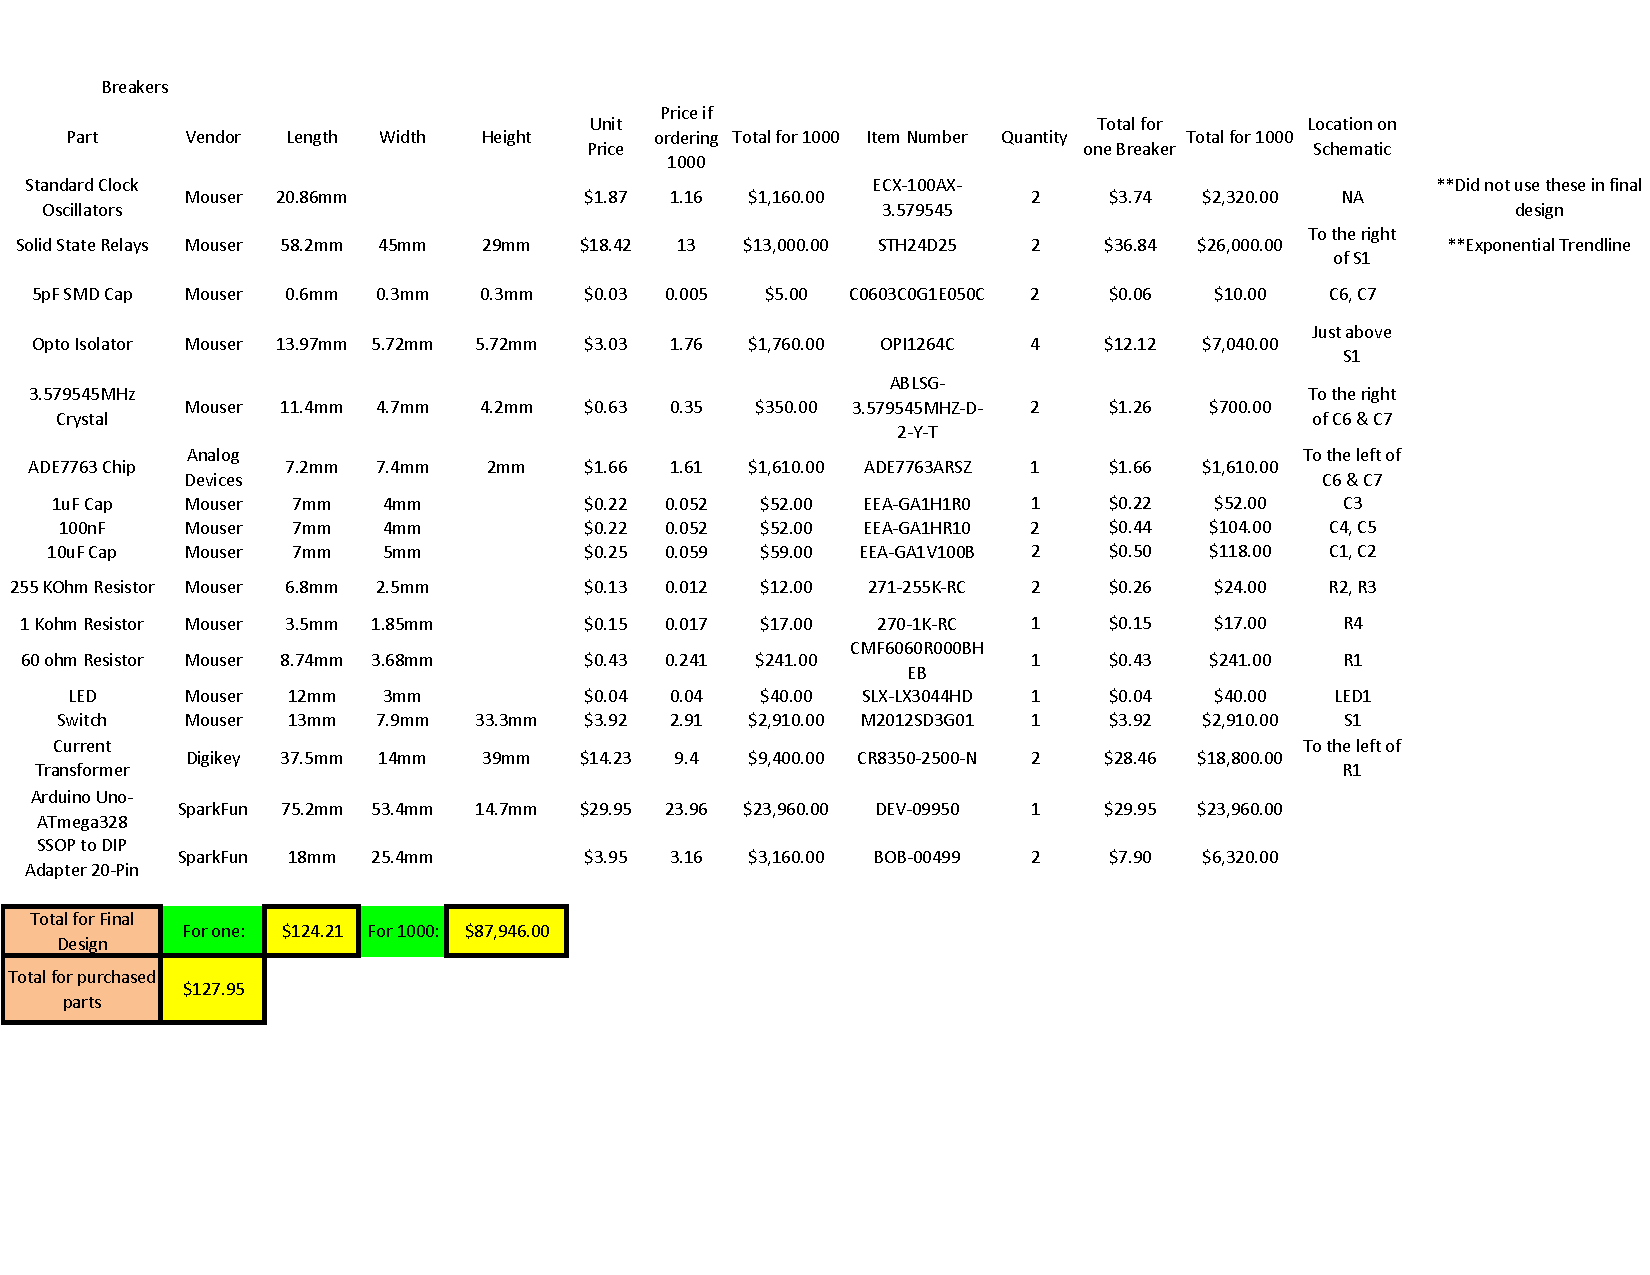
\includegraphics{BillofMaterials_ver5_breakerAdjust.pdf}
% TODO: LaTeX the BoM!!
%Column A: This column was for the part that was purchased.

%Column B: This column was where the part came from and this vendor is where the price reference came from.

%Column C, D, and E: These columns are used for the dimensions. These dimensions were found from mouser, or if mouser did not provide them then they were found from the datasheet of the part. This was used to create a Visio drawing in order to see what a minimum board layout would be. 

%Column F: The price if only one part was to be purchased.

%Column G: This column was used to see if we were to go into production and build 1000, how much would we pay for each part. 

%Column H: Total for 1000 of the parts specified. 

%Column I: The Manufacturer part number. 

%Column J: The quantity that was purchased by our team.

%Column K: Price if we were to only build one full unit based on the quantity purchased.

%Column L: Price if we were to build 1000 units so this was found by (quantity*Price for 1000*1000)

%Column M: Where these parts can be found on the schematic.	

%Column O: Notes that were needed, such as how the price for 1000 was found or wether or not the part was going to be used in the final design.

%At the bottom of the page are totals. These totals are both for 1 unit and the price if we were to build 1000. The price for the final design are only for the parts that were used. The total for all parts are for all the parts that were purchased, but some were not used in the final design.

\begin{figure}[htbp]
\begin{center}
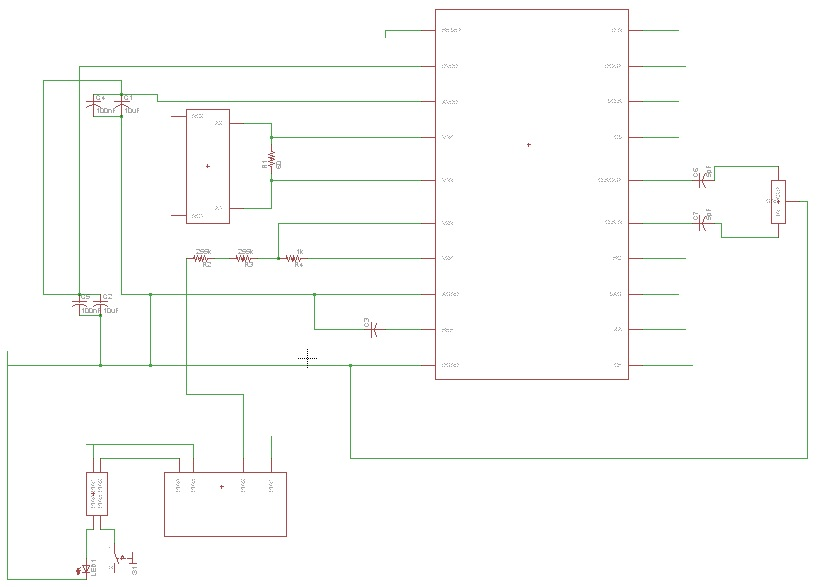
\includegraphics[width=\textwidth]{includes/NJADESchematic} 
\caption{Schematic for Smart Breakers}
\label{fig:ade_schematic}   
\end{center}
\end{figure}

Figure \ref{fig:ade_schematic} is the first version of the smart breaker schematic as drawn in Eagle. Component values were selected as specified in the Component Selection section above. The clock and C1-C5 were specified by the ADE7763 datasheet \cite{ADE7763} and C6 and C7 are specified by the clock datasheet \cite{nateClock}. Changes were made to the optocoupler after the board was printed after recognizing the improper connections. For version 2, pin 1 of the optocoupler was connected to a power source instead of the control line for the solid state relay and $R_{1}$ changed to $42 \ohm$ to account for a larger safety factor. The board and schematic were not changed following the redesigning since the team was using vectorboard for the second version. The schematic does not include the microcontroller since the team decided to locate it off-board so it could be reused later. 

\begin{figure}[htbp]
\begin{center}
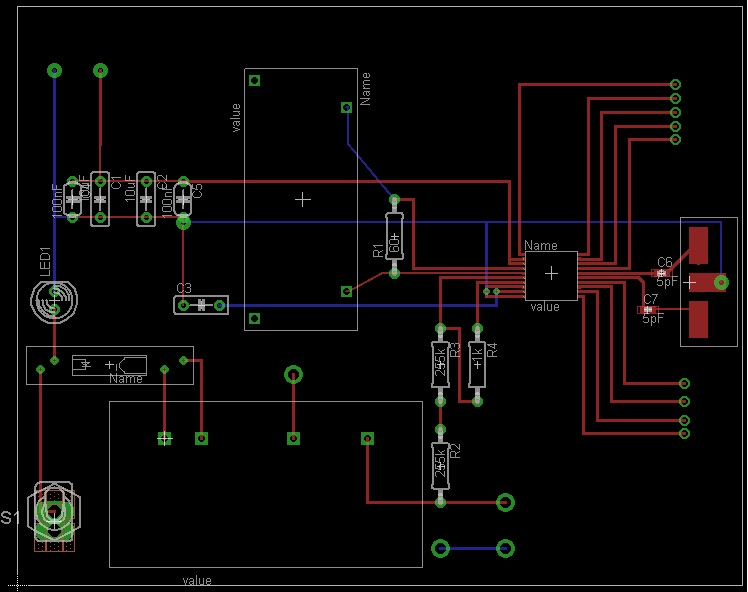
\includegraphics[width=\textwidth]{includes/NJADELayout} 
\caption{PCB layout for Smart Breakers}
\label{fig:ade_layout}   
\end{center}
\end{figure}

Figure \ref{fig:ade_layout} is the first version of the smart breaker layout for a printed circuit board as drawn in Eagle. Little consideration was given to minimizing board space since getting used to Eagle and making all the connections was more important. The ADE7763, solid state relay, current transformer, clock and optocoupler were defined by the team, following the guidelines at instructables.com \cite{instructables}. The microcontroller is again not included due to it's off-board location. 

For the second version of the board, a few changes would be made including a much more compact design with more complicated traces to minimize cost. Also, more traces would be put on the bottom layer to make soldering easier. The team would also use larger traces and pads for connections to the 120 V to handle higher currents. 

\subsubsection{Testing}
%Inputs to ADE7763
The table and graph below show the results of current transformer testing, during which a $6.2\kilo\ohm$ burden resistor was used instead of the $42 \ohm$ selected for final design. This made it easier to read results using an oscilloscope but significantly limited the current threshold as specified by equation \ref{eq:current_safety}. Table \ref{tab:measured_secondaryPercentError} gives the component values used and the resulting voltage and current measurements, both with percent error from values calculated based on measurements on the primary side. Table \ref{tab:measured_primary} shows the inputs used to obtain data for table \ref{tab:measured_secondaryPercentError}. From the data the team confirmed that the current transformer provides a linear relationship between primary and secondary current, and concluded that the chip should be able to read accurately with minimal correction factors. Figure \ref{fig:current_transformers_iv_response} shows this relationship graphically.

\begin{table}[htdp]
\caption{Measured:Primary}
\begin{center}
\begin{tabular}{|c|c|c|c|} \hline
Voltage($\volt$) & Power ($\watt$) & Resistance ($\ohm$) & Current ($\ampere$) \\ \hline
117 & 40.00 & 342 & 0.360 \\ \hline
117 & 20.00 & 684 & 0.250 \\ \hline
117 & 13.33 & 1027 & 0.210 \\ \hline
117 & 10.00 & 1369 & 0.200 \\ \hline
117 & 80.00 & 171 & 0.690 \\ \hline
\end{tabular}
\end{center}
\label{tab:measured_primary}
\end{table}%

\begin{table}[htdp]
\caption{Measured:Secondary with Percent Error}
\begin{center}
\begin{tabular}{|c|c|c|c|c|} \hline
Voltage($\volt$) & \% Error & Resistance ($\ohm$) & Current ($\milli\ampere$) & \% Error \\ \hline
0.840 & 5.5 & 6200 & 0.135 & 5.8 \\ \hline
0.580 & 6.0 & 6200 & 0.093 & 6.6 \\ \hline
0.490 & 5.5 & 6200 & 0.084 & 0.4 \\ \hline
0.440 & 10.9 &6200 & 0.069 & 13.4 \\ \hline
1.620 & 4.9 & 6200 & 0.265 & 3.6 \\ \hline
\end{tabular}
\end{center}
\label{tab:measured_secondaryPercentError}
\end{table}%

\begin{figure}[htbp]
\begin{center}
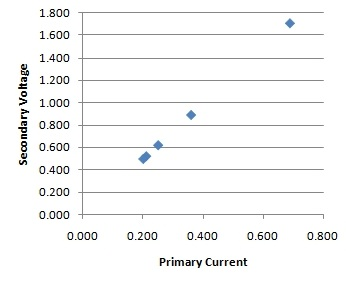
\includegraphics[width=4in]{includes/NJGraph2}
\caption{Current-Voltage Response of Current Transformers}
\label{fig:current_transformers_iv_response}
\end{center}
\end{figure}

\begin{figure}[htbp]
\begin{center}
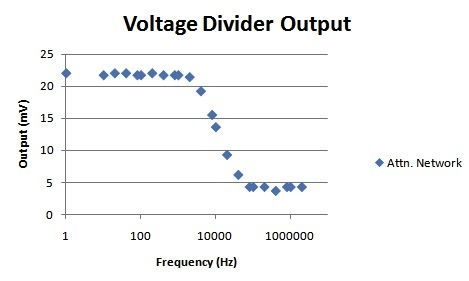
\includegraphics[width=4in]{includes/NJVoltDivOutput}
\caption{Graph showing results from voltage divider testing}
\label{fig:voltage_divider_testing}
\end{center}
\end{figure}

Figure \ref{fig:voltage_divider_testing} shows the results of testing the low pass filter on channel 1 of the ADE7763 metering chip. From the results, the team concluded that the low pass filter works as expected, giving a corner frequency of approximately 10kHz as recommended by the datasheet \cite{ADE7763} to prevent aliasing. 

% Final Decisions follows here

% Future Work is next
